\chapter{Random Forests}\label{ch:forest}

\begin{remark}{Outline}
In this chapter, we present the well-known family of \textit{Random Forests}
methods. In Section~\ref{sec:4:bias-variance}, we first describe the
bias-variance decomposition of the prediction error and then present, in
Section~\ref{sec:4:ensemble}, how aggregating randomized models through
ensembles reduces the prediction error by decreasing the variance term in this
decomposition. In Section~\ref{sec:4:random-forests}, we revisit Random Forests ant its variants and
study how randomness introduced into the decision tree induction algorithm can
reduce prediction error by decorrelating the decision trees in the ensemble.
Finally, the consistency of forests of randomized trees is explored in
Section~\ref{sec:4:consistency}.
\end{remark}

\section{Bias-variance decomposition}
\label{sec:4:bias-variance}

In section~\ref{sec:2:performance-evaluation}, we defined the generalization
error of a model $\varphi_{\cal L}$ as its expected prediction error
according to some loss function $L$
\begin{equation}
Err(\varphi_{\cal L}) = \mathbb{E}_{X,Y} \{ L(Y, \varphi_{\cal L}(X)) \}.
\end{equation}
Similarly, the expected prediction error of $\varphi_{\cal L}$ at $X=\mathbf{x}$
can be expressed as
\begin{equation}
Err(\varphi_{\cal L}(\mathbf{x})) = \mathbb{E}_{Y|X=\mathbf{x}} \{ L(Y, \varphi_{\cal L}(\mathbf{x})) \}.\label{eqn:4:generalization-error:x}
\end{equation}

In regression, this latter form of the expected prediction error additively
decomposes into bias and variance terms which together constitute a very useful
framework for diagnosing the prediction error of a model. In classification, a
similar decomposition is more difficult to obtain. Yet, the
concepts of bias and variance can be transposed in several ways to
classification, thereby providing comparable frameworks for studying the
prediction error of classifiers.

\subsection{Regression}
\label{sec:bias-variance:regression}

In regression, assuming that $L$ is the squared error loss, the expected
prediction error of a model $\varphi_{\cal L}$ at a given point $X=\mathbf{x}$
can be rewritten with respect to the Bayes model $\varphi_B$:
\begin{align}
& Err(\varphi_{\cal L}(\mathbf{x})) \nonumber \\
&= \mathbb{E}_{Y|X=\mathbf{x}} \{ (Y - \varphi_{\cal L}(\mathbf{x}))^2 \} \nonumber \\
&= \mathbb{E}_{Y|X=\mathbf{x}} \{ (Y -\varphi_B(\mathbf{x}) + \varphi_B(\mathbf{x}) - \varphi_{\cal L}(\mathbf{x}))^2 \} \nonumber \\
&= \mathbb{E}_{Y|X=\mathbf{x}} \{ (Y -\varphi_B(\mathbf{x}))^2  \} + \mathbb{E}_{Y|X=\mathbf{x}} \{ (\varphi_B(\mathbf{x}) - \varphi_{\cal L}(\mathbf{x}))^2 \} \nonumber \\
& \quad+ \mathbb{E}_{Y|X=\mathbf{x}} \{ 2 (Y - \varphi_B(\mathbf{x}))(\varphi_B(\mathbf{x}) - \varphi_{\cal L}(\mathbf{x})) \} \nonumber \\
&= \mathbb{E}_{Y|X=\mathbf{x}} \{ (Y -\varphi_B(\mathbf{x}))^2 \} + \mathbb{E}_{Y|X=\mathbf{x}} \{ (\varphi_B(\mathbf{x}) - \varphi_{\cal L}(\mathbf{x}))^2 \} \nonumber \\
&= Err(\varphi_B(\mathbf{x})) +  (\varphi_B(\mathbf{x}) - \varphi_{\cal L}(\mathbf{x}))^2 \label{eqn:4:decomp1}
\end{align}
since $\mathbb{E}_{Y|X=\mathbf{x}} \{ Y - \varphi_B(\mathbf{x}) \} =
\mathbb{E}_{Y|X=\mathbf{x}} \{ Y \} - \varphi_B(\mathbf{x}) = 0$ by definition
of the Bayes model in regression. In this form, the first term in the last
expression of Equation~\ref{eqn:4:decomp1} corresponds to the (irreducible)
residual error  at $X=\mathbf{x}$ while the second term represents the
discrepancy of $\varphi_{\cal L}$ from the Bayes model. The further from the
Bayes model, the more sub-optimal the model and the larger the error.

If we further assume that the learning set ${\cal L}$ is itself a random
variable (sampled from the population $\Omega$) and that the learning algorithm is deterministic, then the expected
discrepancy with the Bayes model can further be re-expressed in terms of the
average prediction $\mathbb{E}_{\cal L} \{ \varphi_{\cal L}(\mathbf{x}) \}$
over the models learned from all possible learning sets of size $N$:
\begin{align}
& \mathbb{E}_{\cal L} \{ (\varphi_B(\mathbf{x}) - \varphi_{\cal L}(\mathbf{x}))^2 \}\nonumber \\
&= \mathbb{E}_{\cal L} \{ (\varphi_B(\mathbf{x}) - \mathbb{E}_{\cal L} \{ \varphi_{\cal L}(\mathbf{x}) \} + \mathbb{E}_{\cal L} \{ \varphi_{\cal L}(\mathbf{x}) \} - \varphi_{\cal L}(\mathbf{x}))^2 \} \nonumber \\
&= \mathbb{E}_{\cal L} \{ (\varphi_B(\mathbf{x}) - \mathbb{E}_{\cal L} \{ \varphi_{\cal L}(\mathbf{x}) \} )^2 \} + \mathbb{E}_{\cal L} \{ (\mathbb{E}_{\cal L} \{ \varphi_{\cal L}(\mathbf{x}) \} - \varphi_{\cal L}(\mathbf{x}))^2 \} \}\nonumber \\
& \quad+ \mathbb{E}_{\cal L} \{ 2(\varphi_B(\mathbf{x}) - \mathbb{E}_{\cal L} \{ \varphi_{\cal L}(\mathbf{x}) \})(\mathbb{E}_{\cal L} \{ \varphi_{\cal L}(\mathbf{x}) \} - \varphi_{\cal L}(\mathbf{x}))\} \nonumber \\
&= \mathbb{E}_{\cal L} \{ (\varphi_B(\mathbf{x}) - \mathbb{E}_{\cal L} \{ \varphi_{\cal L}(\mathbf{x}) \} )^2 \} + \mathbb{E}_{\cal L} \{ (\mathbb{E}_{\cal L} \{ \varphi_{\cal L}(\mathbf{x}) \} - \varphi_{\cal L}(\mathbf{x}))^2 \} \}\nonumber \\
&= (\varphi_B(\mathbf{x}) - \mathbb{E}_{\cal L} \{ \varphi_{\cal L}(\mathbf{x}) \} )^2 + \mathbb{E}_{\cal L} \{ (\mathbb{E}_{\cal L} \{ \varphi_{\cal L}(\mathbf{x}) \} - \varphi_{\cal L}(\mathbf{x}))^2 \}
\end{align}
since $\mathbb{E}_{\cal L}\{ \mathbb{E}_{\cal L} \{ \varphi_{\cal
L}(\mathbf{x}) \} - \varphi_{\cal L}(\mathbf{x}) \} =  \mathbb{E}_{\cal L} \{
\varphi_{\cal L}(\mathbf{x}) \} -  \mathbb{E}_{\cal L} \{ \varphi_{\cal
L}(\mathbf{x}) \} = 0$. In summary, the expected generalization error additively
decomposes as formulated in Theorem~\ref{thm:bias-variance}.

\begin{theorem}\label{thm:bias-variance}
For the square error loss, the bias-variance decomposition of the expected
generalization error $\mathbb{E}_{\cal L} \{ Err(\varphi_{\cal L}(\mathbf{x}))
\}$ at $X=\mathbf{x}$ is
\begin{equation}
\mathbb{E}_{\cal L} \{ Err(\varphi_{\cal L}(\mathbf{x})) \} = \text{noise}(\mathbf{x}) + \text{bias}^2(\mathbf{x}) + \text{var}(\mathbf{x}),
\end{equation}
where
\begin{align}
\text{noise}(\mathbf{x}) &= Err(\varphi_B(\mathbf{x})), \\
\text{bias}^2(\mathbf{x}) &= (\varphi_B(\mathbf{x}) - \mathbb{E}_{\cal L} \{ \varphi_{\cal L}(\mathbf{x}) \} )^2, \\
\text{var}(\mathbf{x}) &= \mathbb{E}_{\cal L} \{ (\mathbb{E}_{\cal L} \{ \varphi_{\cal L}(\mathbf{x}) \} - \varphi_{\cal L}(\mathbf{x}))^2 \}.
\end{align}
\end{theorem}

This bias-variance decomposition of the generalization error is due to
\citet{geman:1992} and was first proposed in the context of neural networks.
The first term, $\text{noise}(\mathbf{x})$, is the residual error. It is
entirely independent of both the learning algorithm and the learning set and
provides for any model a theoretical lower bound on its generalization error.
The second term, $\text{bias}^2(\mathbf{x})$, measures the discrepancy between
the average prediction and the prediction of the Bayes model. Finally, the
third term, $\text{var}(\mathbf{x})$, measures the variability of the
predictions at $X=\mathbf{x}$ over the models learned from all possible
learning sets. All three terms are illustrated in Figure~\ref{fig:bias-variance}
for a toy regression problem. Both $\text{noise}(\mathbf{x})$ and
$\text{var}(\mathbf{x})$ measures the spread of the two densities while
$\text{bias}^2(\mathbf{x})$ is the distance between their means.

\begin{figure}
    \centering
    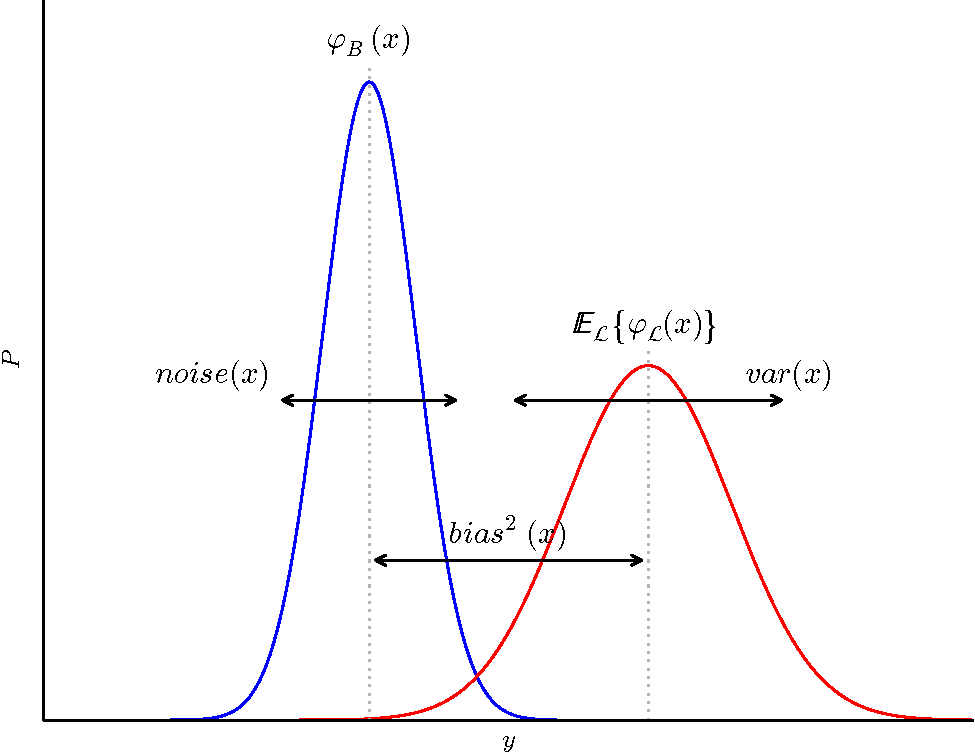
\includegraphics[width=0.9\textwidth]{figures/ch4_bias_variance.pdf}
    \caption{Residual error, bias and variance at $X=\mathbf{x}$. (Figure inspired from \citep{geurts:2002}.)}
    \label{fig:bias-variance}
\end{figure}

As a typical example, the bias-variance decomposition framework can be used as
a tool for diagnosing underfitting and overfitting (as previously introduced in
Section \ref{sec:2:model-selection}). The upper plots in
Figure~\ref{fig:overfitting} illustrate in light red predictions $\varphi_{\cal
L}(\mathbf{x})$ for polynomials of degree $1$, $5$ and $15$ learned over random
learning sets ${\cal L}$ sampled from a noisy cosinus function. Predictions
$\mathbb{E}_{\cal L} \{ \varphi_{\cal L}(\mathbf{x}) \}$ of the average model
are represented by the thick red lines. Predictions for the model learned over
the learning set represented by the blue dots are represented in gray.
Predictions of the Bayes model are shown in blue and coincide with the unnoised
cosinus function that defines the regression problem. The lower plots in the
figure illustrate the bias-variance decomposition of the expected
generalization error of the polynomials.

\begin{figure}
    \hspace{-0.75cm}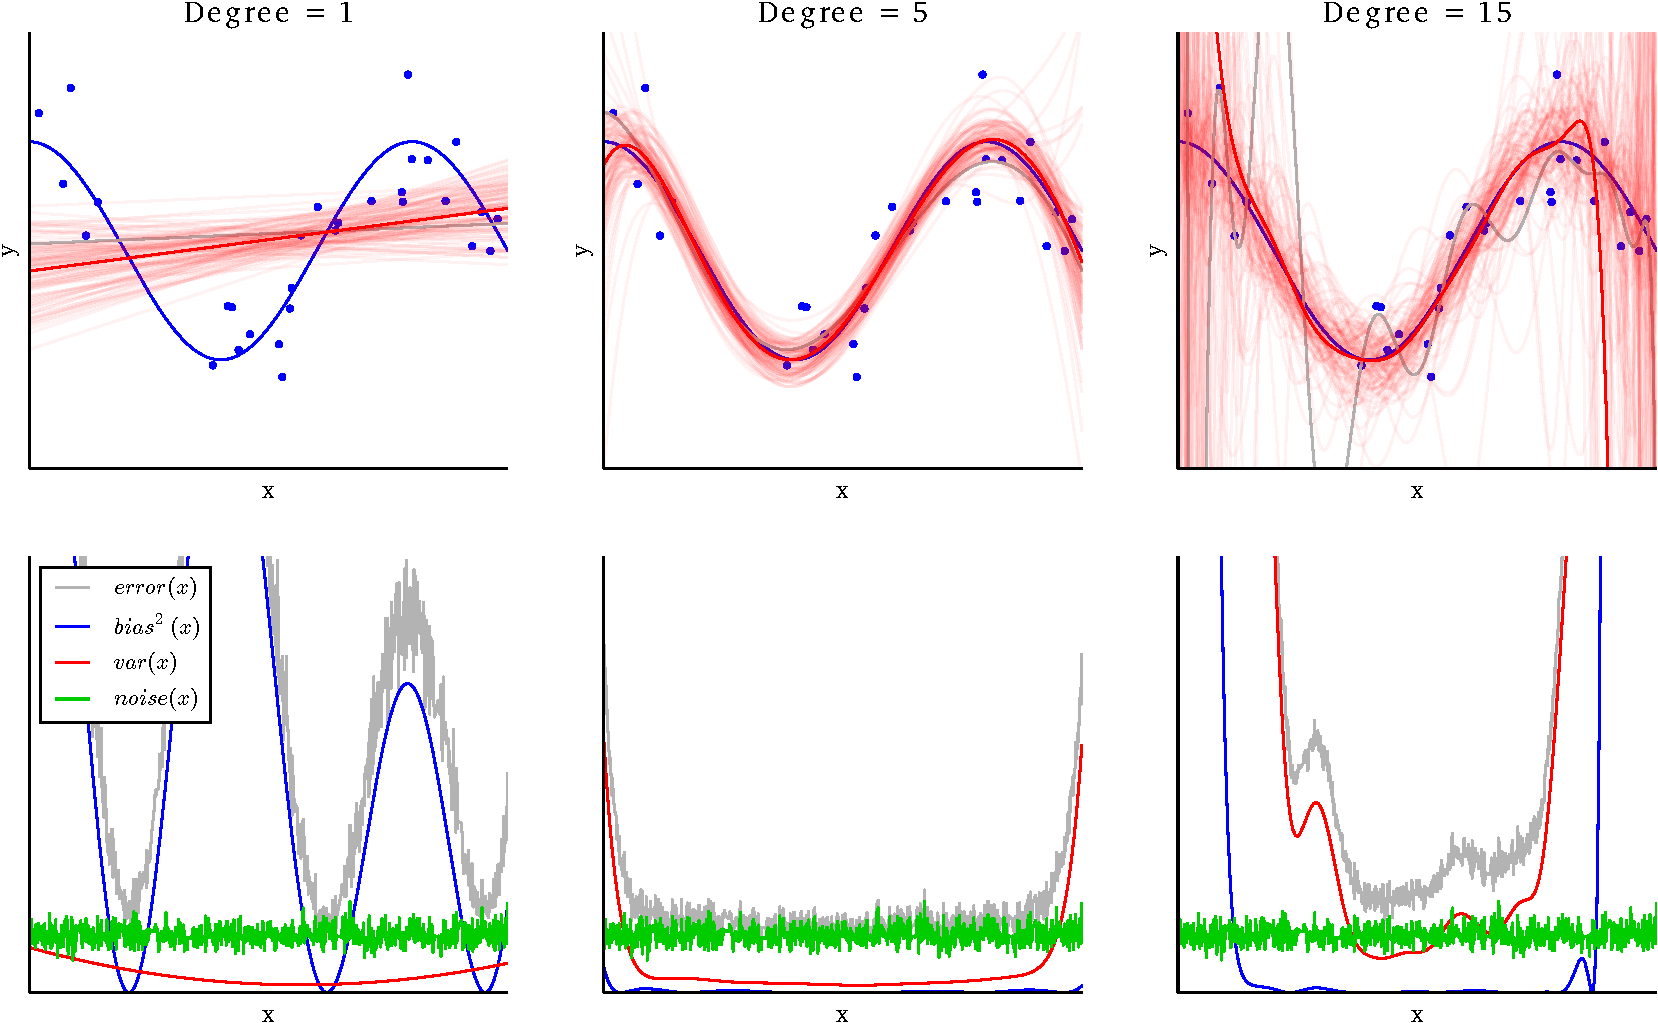
\includegraphics[width=1.1\textwidth]{figures/ch4_overfitting.pdf}
    \caption{Bias-variance decomposition of the expected generalization error for polynomials of degree $1$, $5$ and $15$.}
    \label{fig:overfitting}
\end{figure}

Clearly, polynomials of degree $1$ (left) suffer from underfitting. In terms of
bias and variance, this translates into low variance but high bias as shown in
the lower left plot of Figure~\ref{fig:overfitting}. Indeed, due to the low
degree of the polynomials (i.e., due to the low model complexity), the
resulting models are almost all identical and  the variability of the
predictions from one model to another is therefore quite low. Also, because of
low complexity, none of them really fits the trend of the training points, even
approximately, which implies that the average model is far from approximating
the Bayes model. This results in high bias. On the other hand, polynomials of
degree $15$ (right) suffer from overfitting. In terms of bias and variance, the
situation is the opposite. Predictions have low bias but high variance, as
shown in the lower right plot of Figure~\ref{fig:overfitting}. The variability
of the predictions is large because the high degree of the polynomials (i.e.,
the high model complexity) captures noise in the learning set. Indeed, compare
the gray line with the blue dots -- they almost all intersect. Put otherwise,
small changes in the learning set result in large changes in the obtained model
and therefore in its predictions. By contrast, the average model is now quite
close from the Bayes model, which results in low bias\footnote{Note however the
Gibbs-like phenomenon resulting in both high variance and high bias at the
boundaries of ${\cal X}$.}. Finally, polynomials of degree $5$ (middle) are
neither too simple nor too complex. In terms of bias and variance, the trade-
off is well-balanced between the two extreme situations. Bias and variance are
neither too low nor too large.

\subsection{Classification}
\label{sec:bias-variance:classification}

In direct analogy with the bias-variance decomposition for the square error
loss, similar decompositions have been proposed in the literature for the
expected generalization error based on the zero-one loss, i.e., for
$\mathbb{E}_{\cal L}\{ \mathbb{E}_{Y|X=\mathbf{x}} \{ 1(\varphi_{\cal L}(x)
\neq Y) \} \} = P_{{\cal L},Y|X=\mathbf{x}}(\varphi_{\cal L}(\mathbf{x}) \neq
Y)$. Most notably, \citet{dietterich:1995}, \citet{breiman:1996},
\citet{kohavi:1996} and \citet{tibshirani:1996} have all developed additive
decompositions similar to Theorem~\ref{thm:bias-variance} by redefining the
concepts of bias and variance in the case of classification. While these
efforts have all provided useful insight into the nature of classification
error, none of them really have provided a seductively as simple and
satisfactory framework as in regression (for reviews, see
\citep{friedman:1997,geurts:2002,james:2003}).

An interesting connection with Theorem~\ref{thm:bias-variance} however is to
remark that classification algorithms usually work by computing estimates
\begin{equation}
p_{\cal L}(Y=c|X=\mathbf{x})
\end{equation}
of the conditional class probability (e.g.,
$p_{\cal L}(Y=c|X=\mathbf{x}) = p(c|t)$ in decision trees, where $t$ is the
leaf reached by $\mathbf{x}$) and then deriving a classification rule by
predicting the class that maximizes this estimate, that is:
\begin{equation}\label{eqn:4:classificaton-rule}
\varphi_{\cal L}(\mathbf{x}) = \argmax_{c \in {\cal Y}} p_{\cal L}(Y=c|X=\mathbf{x})
\end{equation}
As such, a direction for studying classification models is the relate the
bias-variance decomposition of these numerical estimates to the expected
misclassification error of classification rule~\ref{eqn:4:classificaton-rule}.

We now reproduce the results of \citet{friedman:1997} who made this connection
explicit for the case of binary classification. Let us first decompose the
expected classification error into an irreducible part associated with the
random nature of the output $Y$ and a reducible part that depends on
$\varphi_{\cal L}(\mathbf{x})$, in analogy with Equation~\ref{eqn:4:decomp1}
for the square error loss. (Note that, to simplify notations, we assume that
all probabilities based on the random variable $Y$ is with respect to the
distribution of $Y$ at $X=\mathbf{x}$.)
\begin{align}
& \mathbb{E}_{\cal L}\{ \mathbb{E}_{Y|X=\mathbf{x}} \{ 1(\varphi_{\cal L}(x) \neq Y) \} \}  \\
&= P_{{\cal L}}(\varphi_{\cal L}(\mathbf{x}) \neq Y) \nonumber \\
&= \begin{aligned}[t]
    1 &- P_{\cal L}(\varphi_{\cal L}(\mathbf{x}) = \varphi_B(\mathbf{x})) P(\varphi_B(\mathbf{x})=Y) \nonumber \\
      &- P_{\cal L}(\varphi_{\cal L}(\mathbf{x}) \neq \varphi_B(\mathbf{x})) P(\varphi_B(\mathbf{x})\neq Y) \nonumber
   \end{aligned}\nonumber \\
&= \begin{aligned}[t]
    &P(\varphi_B(\mathbf{x})\neq Y) + P_{\cal L}(\varphi_{\cal L}(\mathbf{x})\neq \varphi_B(\mathbf{x})) \nonumber \\
    &- 2 P_{\cal L}(\varphi_{\cal L}(\mathbf{x})\neq \varphi_B(\mathbf{x})) P(\varphi_B(\mathbf{x})\neq Y)  \nonumber \\
   \end{aligned}\nonumber \\
&= P(\varphi_B(\mathbf{x})\neq Y) + P_{\cal L}(\varphi_{\cal L}(\mathbf{x})\neq \varphi_B(\mathbf{x}))(2 P(\varphi_B(\mathbf{x}) = Y) - 1) \nonumber
\end{align}

In this form, the first term is the irreducible error of the Bayes model. The
second term is the increased error due to the misestimation of the optimal
decision boundary. The probability $P_{\cal L}(\varphi_{\cal L}(\mathbf{x})\neq
\varphi_B(\mathbf{x}))$  is the probability for the model of making a decision
which is different from the decision of the Bayes model. This happens
when the estimate $p_{\cal L}(Y=\varphi_B(\mathbf{x}))$ is lower
than $0.5$, that is:
\begin{equation}\label{eqn:4:prob-diff-from-bayes}
P_{\cal L}(\varphi_{\cal L}(\mathbf{x})\neq \varphi_B(\mathbf{x})) = P_{\cal L}(p_{\cal L}(Y=\varphi_B(\mathbf{x})) < 0.5)
\end{equation}
As Figure~\ref{fig:estimate-distribution} illustrates, probability~\ref{eqn:4:prob-diff-from-bayes}
therefore corresponds to the tail area on the left side
of the decision threshold (at 0.5) of the distribution of the estimate.

\begin{figure}
    \centering
    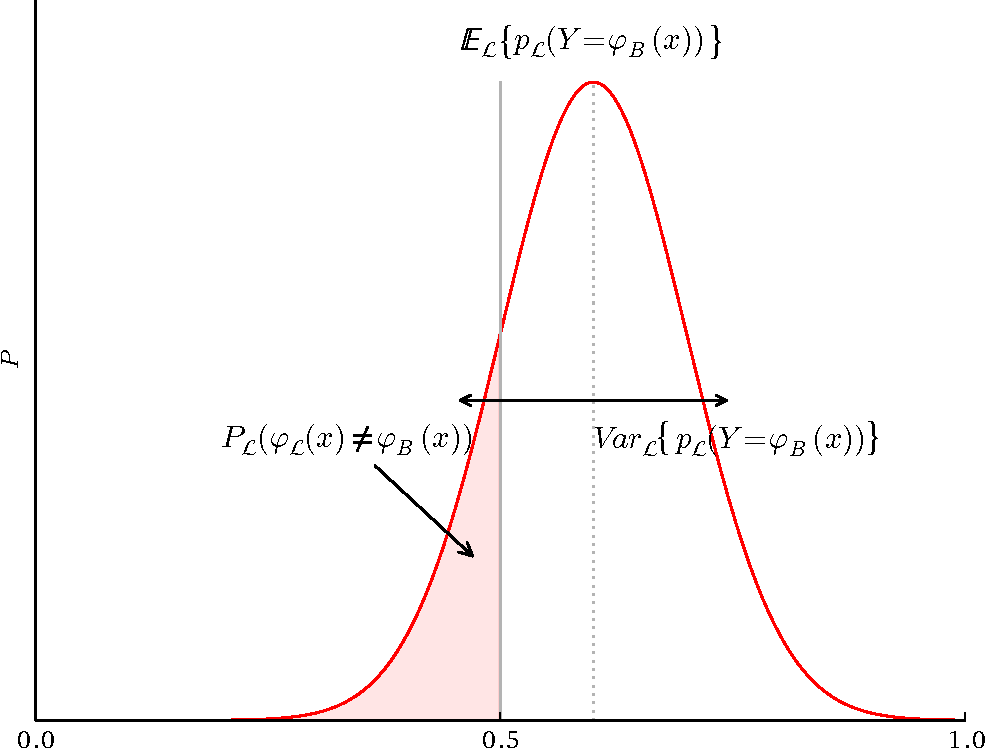
\includegraphics[width=0.9\textwidth]{figures/ch4_estimate_distribution.pdf}
    \caption{Probability distribution of $p_{\cal L}(Y=\varphi_B(\mathbf{x}))$.}
    \label{fig:estimate-distribution}
\end{figure}

If we now further assume\footnote{For single decision trees, the normal
assumption is certainly not satisfied in all cases, but the qualitative
conclusions are still generally valid. When the computations of the estimates
involve some averaging process, e.g., as further developed in the case of
ensemble of randomized trees, this approximation is however fairly reasonable.}
that the estimate $p_{\cal L}(Y=\varphi_B(\mathbf{x}))$ is normally distributed,
then probability~\ref{eqn:4:prob-diff-from-bayes} can be computed explicitly
from its mean and variance:
\begin{equation}
P_{\cal L}(p_{\cal L}(Y=\varphi_B(\mathbf{x})) < 0.5) = \Phi(\frac{0.5 - \mathbb{E}_{\cal L}\{ p_{\cal L}(Y=\varphi_B(\mathbf{x})) \}}{\sqrt{\text{Var}_{\cal L}\{ p_{\cal L}(Y=\varphi_B(\mathbf{x})) \}}})
\end{equation}
where $\Phi(x)=\frac{1}{\sqrt{2\pi}} \int_{-\infty}^x \exp(-\frac{t^2}{2}) dt$
is the cumulative distribution function of the standard normal distribution.
In summary, the expected generalization error additively
decomposes as formulated in Theorem~\ref{thm:bias-variance:classification}.

\begin{theorem}\label{thm:bias-variance:classification}
For the zero-one loss and binary classification, the expected
generalization error $\mathbb{E}_{\cal L} \{ Err(\varphi_{\cal L}(\mathbf{x}))
\}$ at $X=\mathbf{x}$ decomposes as follows:

\begin{align}
\mathbb{E}_{\cal L} \{ Err(\varphi_{\cal L}(\mathbf{x})) \} &= P(\varphi_B(\mathbf{x})\neq Y) \\
                                                            &+ \Phi(\frac{0.5 - \mathbb{E}_{\cal L}\{ p_{\cal L}(Y=\varphi_B(\mathbf{x})) \}}{\sqrt{\text{Var}_{\cal L}\{ p_{\cal L}(Y=\varphi_B(\mathbf{x})) \}}}) (2 P(\varphi_B(\mathbf{x}) = Y) - 1) \nonumber
\end{align}
\end{theorem}

As a result, Theorem~\ref{thm:bias-variance:classification} establishes a
direct connection between the regression variance of the estimates and the
classification error of the resulting model. In practice, this decomposition
has important consequences:
\begin{itemize}
\item When the expected probability estimate $\mathbb{E}_{\cal L}\{ p_{\cal L}(Y=\varphi_B(\mathbf{x}) \}$
      for the true majority class is greater than $0.5$, a reduction of
      variance of the estimate results in a decrease of the total misclassification
      error. If $\text{Var}_{\cal L}\{ p_{\cal L}(Y=\varphi_B(\mathbf{x})) \} \to 0$,
      then $\Phi \to 0$ and the expected generalization error tends to the error of the Bayes model.
      In particular, the generalization error can be driven to its minimum
      value whatever the regression bias of the estimate (at least as long as $\mathbb{E}_{\cal L}\{ p_{\cal L}(Y=\varphi_B(\mathbf{x}) \} > 0.5$).
\item Conversely, when $\mathbb{E}_{\cal L}\{ p_{\cal L}(Y=\varphi_B(\mathbf{x}) \} < 0.5$,
      a decrease of variance might actually increase the total misclassification error.
      If $\text{Var}_{\cal L}\{ p_{\cal L}(Y=\varphi_B(\mathbf{x})) \} \to 0$,
      then $\Phi \to 1$ and the error is maximal.
\end{itemize}

\section{Ensemble methods}
\label{sec:4:ensemble}

Both theorems~\ref{thm:bias-variance} and \ref{thm:bias-variance:classification}
reveal the role of variance in the expected generalization error of a model. In
light of these results, a sensible approach for reducing generalization error
would therefore consist in driving down the prediction variance, provided the
respective bias can be kept the same or not be increased too much.

As it happens, \textit{ensemble methods} constitute a beautifully simple way to
do just that. Specifically, the core principle of ensemble methods is to
introduce random perturbations into the learning procedure in order to produce
several different models from a single learning set ${\cal L}$ and then to
combine the predictions of those models to form the prediction of the ensemble.
How predictions are combined and why does it help is formally studied in the
next sections.

\subsection{Randomized models}

Given a learning set ${\cal L}$, a learning algorithm ${\cal A}$
deterministically produces a model ${\cal A}(\theta, {\cal L})$, denoted
$\varphi_{{\cal L},\theta}$, where $\theta$ are hyper-parameters controlling
the execution of ${\cal A}$. Let us assume that $\theta$ includes a random seed
parameter for mimicking some stochastic behavior in ${\cal A}$, hence producing
(pseudo-)randomized models that are more or less different from one random seed
to another. (We defer the discussion on specific random perturbations in the
case of decision trees to Section~\ref{sec:4:random-forests}.)

In this context, the bias-variance decomposition can be extended to account for
everything that is random, hence considering both ${\cal L}$ and $\theta$ as
random variables\footnote{From now on, and without loss of generality, we
assume that the random variable $\theta$ only controls the randomness of the
learning algorithm -- and nothing else in the learning algorithm.}.
Accordingly, theorems~\ref{thm:bias-variance} and \ref{thm:bias-variance:classification}
naturally extend to the expected generalization error
$\mathbb{E}_{{\cal L},\theta} \{ Err(\varphi_{{\cal L},\theta}(\mathbf{x})) \}$
of the randomized model $\varphi_{{\cal L},\theta}$ by replacing expectations
$\mathbb{E}_{\cal L} \{ . \}$ and variances $\text{Var}_{\cal L} \{ . \}$ with
their respective counterparts $\mathbb{E}_{{\cal L},\theta} \{ . \}$ and
$\text{Var}_{{\cal L},\theta} \{ . \}$ computed over the joint distribution of
${\cal L}$ and $\theta$. In regression, the bias-variance decomposition
of the square error loss thus becomes:
\begin{equation}
\mathbb{E}_{{\cal L},\theta} \{ Err(\varphi_{{\cal L},\theta}(\mathbf{x})) \} = \text{noise}(\mathbf{x}) + \text{bias}^2(\mathbf{x}) + \text{var}(\mathbf{x}),
\end{equation}
where
\begin{align}
\text{noise}(\mathbf{x}) &= Err(\varphi_B(\mathbf{x})), \\
\text{bias}^2(\mathbf{x}) &= (\varphi_B(\mathbf{x}) - \mathbb{E}_{{\cal L},\theta} \{ \varphi_{{\cal L},\theta}(\mathbf{x}) \} )^2, \\
\text{var}(\mathbf{x}) &= \mathbb{E}_{{\cal L},\theta} \{ (\mathbb{E}_{{\cal L},\theta} \{ \varphi_{{\cal L},\theta}(\mathbf{x}) \} - \varphi_{{\cal L},\theta}(\mathbf{x}))^2 \}.
\end{align}

In this form, variance now accounts for both the prediction variability due to
the randomness of the learning set ${\cal L}$ and the variability due to the
randomness of the learning algorithm itself. As a result, the variance of a
randomized algorithm is usually strictly larger than the variance of its
deterministic counterpart. Depending on the strength of randomization, bias
also usually increases, but usually to a smaller extent than variance.


\subsection{Combining randomized models}

Let us assume a set of $M$ randomized models $\{\varphi_{{\cal L},
\theta_i} | i = 1, \dots, M \}$, all built on the same learning set ${\cal L}$
but each from an independent random seed $\theta_i$.

% Diminiuer la variance réduit l'erreur
% => Faire un ensemble de modèles légèremet différents de l'un à l'autre permet de réduire la variance
% => le montrer et fainre le lien avec correlation
% RF differ from each in the way they decorrelate pairs of trees




\subsection{Bias-variance decomposition of an ensemble}
\label{sec:4:bias-variance:ensemble}

% bias variance of ensemble of randomized
    % Aggregation
    % > consensus vote
    % > average probability (Hastie, 283+)
    % > average output values

% discussion on the correlation coefficient + increase of bias

% RF do not overfit (theorem 2.3)

\section{Random Forests}
\label{sec:4:random-forests}

% \subsubsection{Bagging}
% \subsubsection{Random Forests}
% \subsubsection{Extremely Randomized Trees}

% bagging
% pasting
% random forests algorithms
    % - Bagging
    % - Random features (Kwok & carter (1990), dietterich 1998 (see rf), breiman)
    % - Random thresholds (geurts)
    % - +other kinds of forests (see state-of-the-art in geurts)
    % => discuter sur un exemple les aspects stat/comput/repres
    % Ex: correlation coeff example

% Issues tackled by ensemble
%   Ensemble methods in ML, Dietterich
%   - stat
%   - computational
%   - representational

%\subsection{Byproducts of Random Forests}

% \subsubsection{Out-of-bag estimates}
% \subsubsection{Proximity plots}
% \subsubsection{Variable importances}

\section{Consistency}
\label{sec:4:consistency}

    % > Mise au point
    % > Preuve de consistence des extra-trees?
